%% Version 5.0, 2 January 2020
%
%%%%%%%%%%%%%%%%%%%%%%%%%%%%%%%%%%%%%%%%%%%%%%%%%%%%%%%%%%%%%%%%%%%%%%
% TemplateV5.tex --  LaTeX-based template for submissions to the
% American Meteorological Society
%
%%%%%%%%%%%%%%%%%%%%%%%%%%%%%%%%%%%%%%%%%%%%%%%%%%%%%%%%%%%%%%%%%%%%%
% PREAMBLE
%%%%%%%%%%%%%%%%%%%%%%%%%%%%%%%%%%%%%%%%%%%%%%%%%%%%%%%%%%%%%%%%%%%%%

%% Start with one of the following:
% DOUBLE-SPACED VERSION FOR SUBMISSION TO THE AMS
\documentclass[]{ametsocV5}


% TWO-COLUMN JOURNAL PAGE LAYOUT---FOR AUTHOR USE ONLY
% \documentclass[twocol]{ametsocV5}


% Enter packages here. If too many math alphabets are used,
% remove unnecessary packages or define hmmax and bmmax as necessary.

\newcommand{\hmmax}{0}
\newcommand{\bmmax}{0}
\usepackage{amsmath,amsfonts,amssymb,bm}
\usepackage{mathptmx}%{times}
\usepackage{newtxtext}
\usepackage{newtxmath}

\usepackage{gensymb}

%%%%%%%%%%%%%%%%%%%%%%%%%%%%%%%%

%%% To be entered by author:

%% May use \\ to break lines in title:

\title{Title here}


\authors{Elio Campitelli
\correspondingauthor{Elio Campitelli,elio.campitelli@cima.fcen.uba.ar}
and Leandro Díaz
}

\affiliation{CIMA UBA blablabla}

\extraauthor{Carolina Vera
}


%%%%%%%%%%%%%%%%%%%%%%%%%%%%%%%%%%%%%%%%%%%%%%%%%%%%%%%%%%%%%%%%%%%%%
% ABSTRACT
%
% Enter your abstract here
% Abstracts should not exceed 250 words in length!
%


\abstract{Enter the text of your abstract here. This is a sample American
Meteorological Society (AMS) \LaTeX~template. This document provides
authors with instructions on the use of the AMS \LaTeX~template. Authors
should refer to the file amspaper.tex to review the actual \LaTeX~code
used to create this document. The template.tex file should be modified
by authors for their own manuscript.}

\begin{document}

%% Necessary!
\maketitle

\bibliographystyle{ametsoc2014}
%%%%%%%%%%%%%%%%%%%%%%%%%%%%%%%%%%%%%%%%%%%%%%%%%%%%%%%%%%%%%%%%%%%%%
% SIGNIFICANCE STATEMENT/CAPSULE SUMMARY
%%%%%%%%%%%%%%%%%%%%%%%%%%%%%%%%%%%%%%%%%%%%%%%%%%%%%%%%%%%%%%%%%%%%%
%
% If you are including an optional significance statement for a journal article or a required capsule summary for BAMS
% (see www.ametsoc.org/ams/index.cfm/publications/authors/journal-and-bams-authors/formatting-and-manuscript-components for details),
% please apply the necessary command as shown below:
%
\statement
This is significant becasue I wrote it.



%%%%%%%%%%%%%%%%%%%%%%%%%%%%%%%%%%%%%%%%%%%%%%%%%%%%%%%%%%%%%%%%%%%%%
% MAIN BODY OF PAPER
%%%%%%%%%%%%%%%%%%%%%%%%%%%%%%%%%%%%%%%%%%%%%%%%%%%%%%%%%%%%%%%%%%%%%
%

\section{Introduction}

yada yada SAM yada yada circulation.. yada yada so important. yada yada
many impacts.

\section{Methods}

\subsubsection{Data}

We used monthly geopotential height at 2.5 longitude by 2.5 latitude
resolution from ERA5 \citep{hersbach} for the period 1979 to 2018
(inclusive).

Monthly temperature NOAA Global Surface Temperature (NOAAGlobalTemp) 5.0
degree latitude x 5.0 degree longitude global grid
\citep{vose2012, smith2008}. The same analysis was carried out using
CRUTEM4 \citep{osborn2014} (not shown).

We used monthly precipitation data from CPC Merged Analysis of
Precipitation \citep{xie1997} 2.5 degree latitude x 2.5 degree
longitude.

\subsubsection{Definition of indexes}

We defined the Southern Annular Mode (SAM) as the leading EOF of the
monthly anomalies of geopotential field at 700 hPa south of 20\degree S
(citation?). The EOF was performed by computing the Singular Value
Decomposition of the data matrix consisting in 481 rows and 4176 columns
(144 points of longitude and 29 points of latitude). The values where
weighted by the square root of the cosine of latitude to account for the
non-equal area of each gridpoint \citep{chung1999}. This same method was
used at the rest of the levels considered in this paper.

To separate between the zonally symmetric and asymmetric components of
the SAM, we computed the zonal mean and anomalies of the full SAM
spatial pattern. The results are shown in Figure~\ref{fig:method} for
700hPa. The full spatial signal (\(\mathrm{EOF_1}(\lambda, \phi)\)) is
the sum of the zonally asymmetric (\(\mathrm{EOF_1^*}(\lambda, \phi)\))
and symmetric (\([\mathrm{EOF_1}](\lambda, \phi)\)) components. We then
compute the ``Full'', ``Asymmetric'' and ``Symmetric'' indexes, by
regressing each geopotential field on these patterns (weighting by the
cosine of latitude).

The three indexes are normalised by dividing them by the standard
deviation of the ``Full'' index at each level. This means that comparing
the magnitude between indexes is meaningful, but it also means that not
every index will have unit standard deviation.

\begin{figure*}
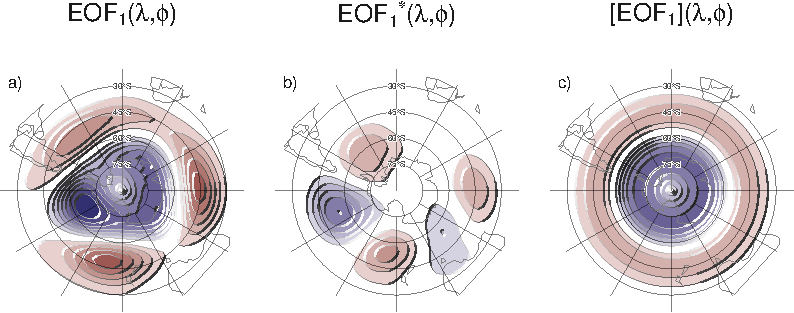
\includegraphics{method-1} \caption[Spatial patterns of the first EOF of 700 hPa geopotential height]{Spatial patterns of the first EOF of 700 hPa geopotential height. Full field (left), zonally asymmetric component (middle) and zonally symmetric component (right). Arbitrary units.}\label{fig:method}
\end{figure*}

\subsubsection{Significance}

We adjusted p-values for False Detection Rate following
\citet{wilks2016}.

\section{Results}

\begin{figure*}
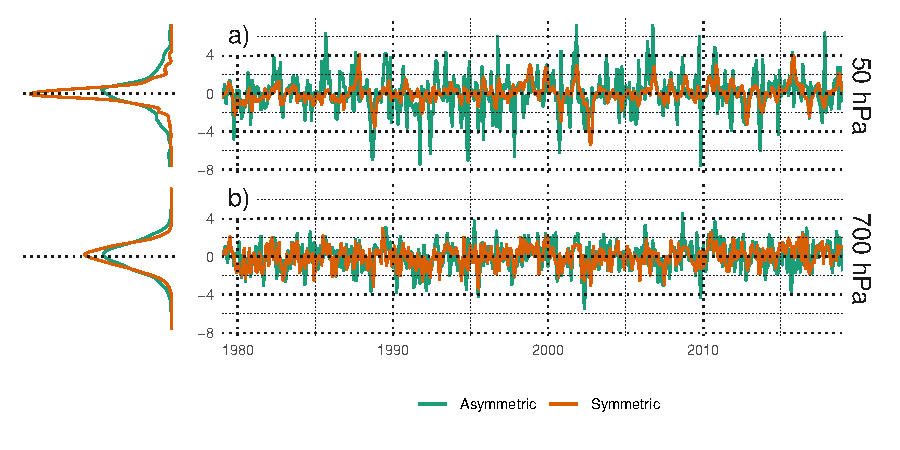
\includegraphics{asymsam-timeseries-1} \caption[Time series for the asymmetric SAM and symmetric SAM]{Time series for the asymmetric SAM and symmetric SAM.}\label{fig:asymsam-timeseries}
\end{figure*}

\begin{figure}
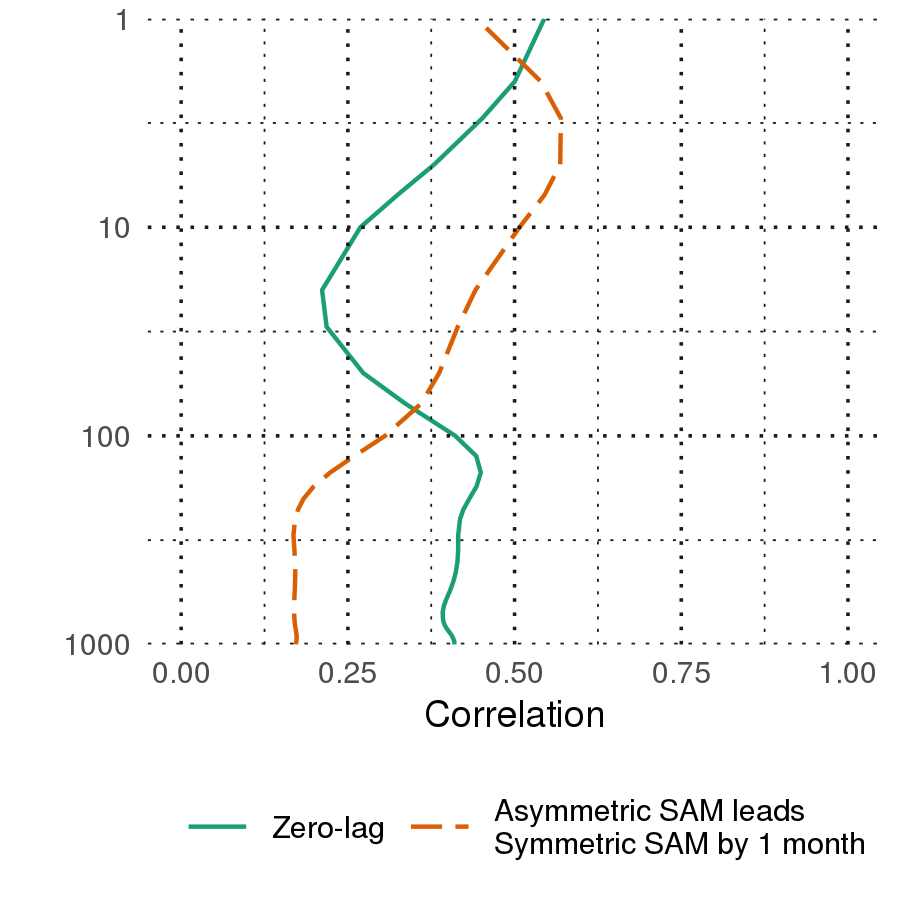
\includegraphics{cor-lev-1} \caption[Correlation between the Symmetric and Asymmetric SAM at each level]{Correlation between the Symmetric and Asymmetric SAM at each level.}\label{fig:cor-lev}
\end{figure}

\begin{figure*}
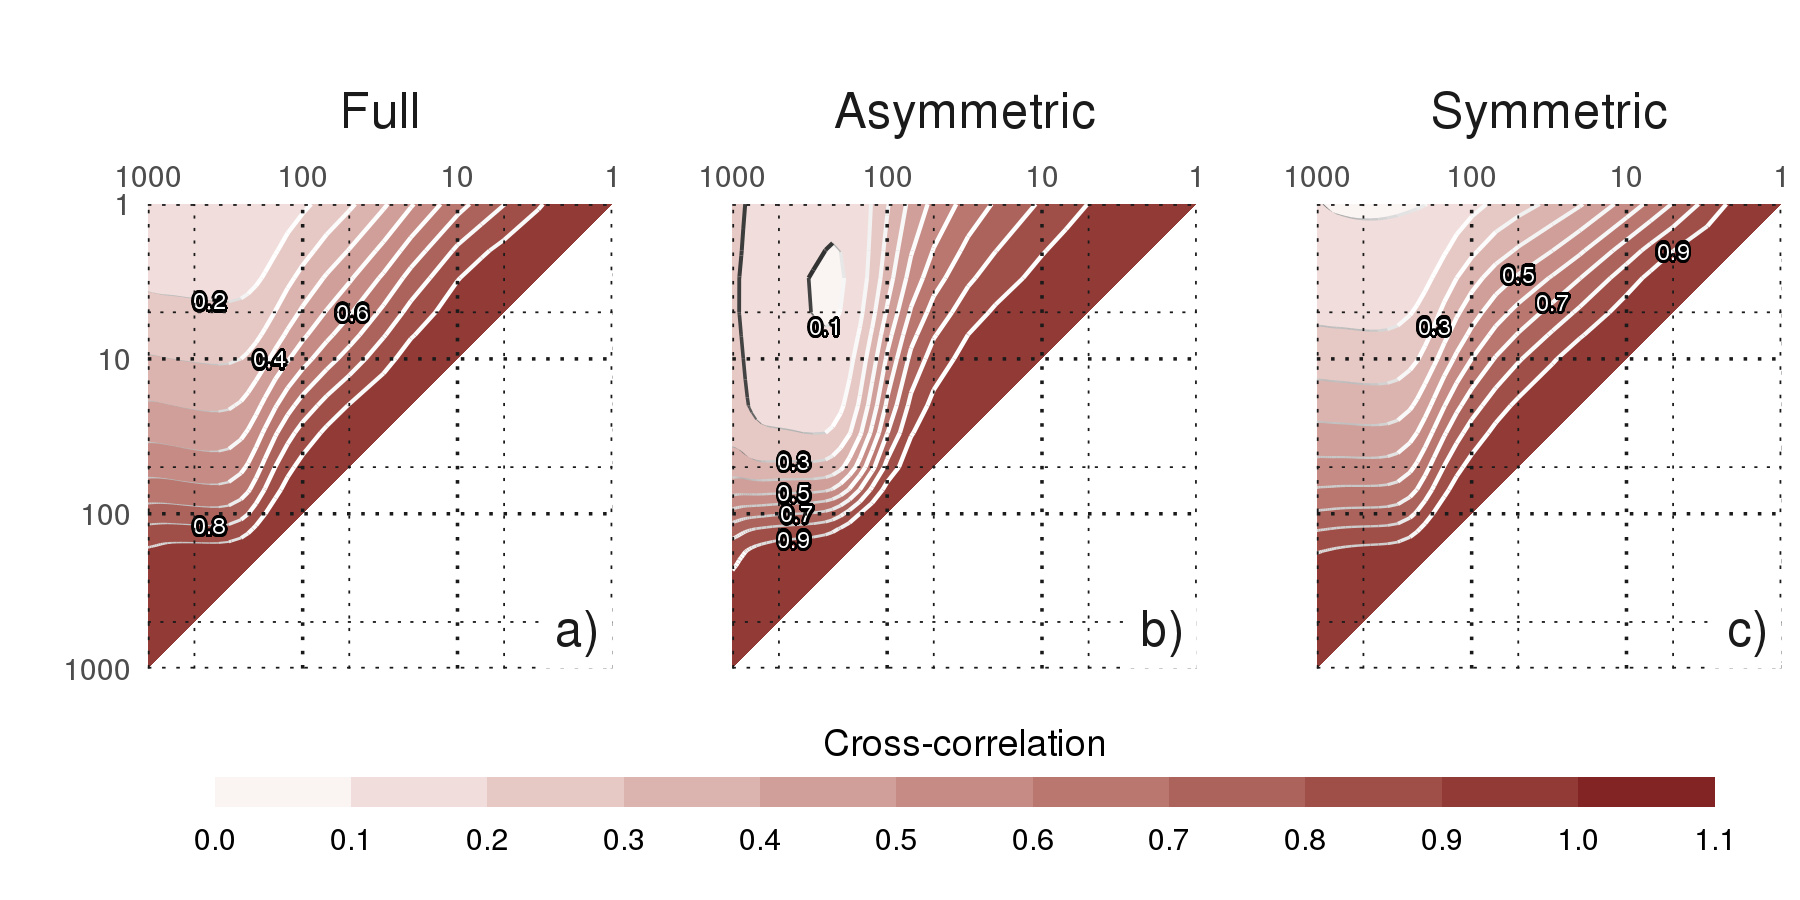
\includegraphics{cross-correlation-1} \caption[Cross correlation between levels of the Full, Asymmetric and Symmetric SAM]{Cross correlation between levels of the Full, Asymmetric and Symmetric SAM.}\label{fig:cross-correlation}
\end{figure*}

\begin{figure*}
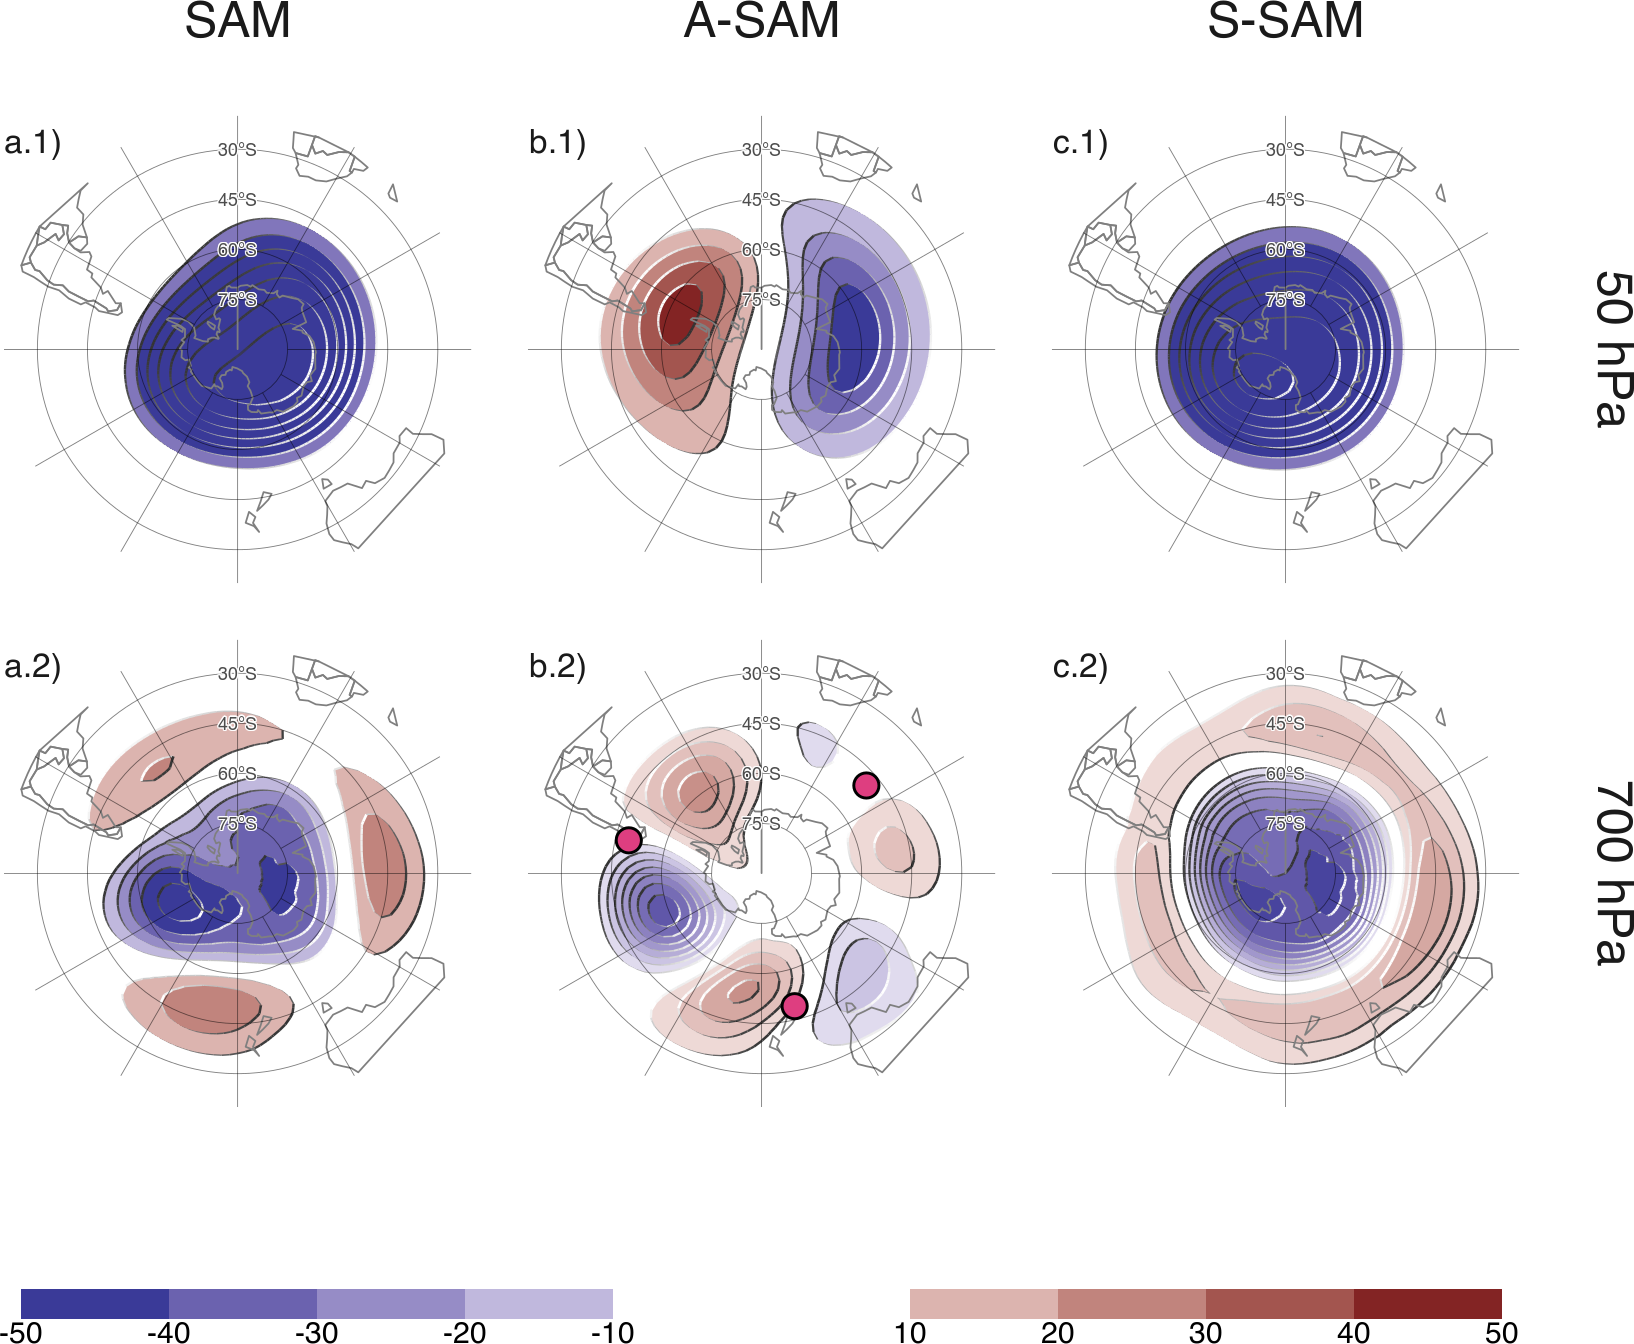
\includegraphics{2d-regr-1} \caption[Regression patterns of geopotential height at 30, 300 and 700 hPa with the Full, Asymmetric and Symmetric SAM]{Regression patterns of geopotential height at 30, 300 and 700 hPa with the Full, Asymmetric and Symmetric SAM. The regression patterns for Asymmetric and Symmetric SAM are the result of one multiple regression using both indices, not of two simple regressions involving each index by itsef.}\label{fig:2d-regr}
\end{figure*}

Sem tortor mus non tristique augue. Donec vel feugiat sit aliquet lorem
dui lobortis dolor risus. Proin, ac eu, mauris. Dolor id habitasse,
curabitur platea ante. Rhoncus volutpat himenaeos vestibulum ut bibendum
felis non. Ligula placerat ac luctus ad. Ante, lorem volutpat eu dapibus
pharetra arcu. Sollicitudin eu tortor amet. Maecenas nulla euismod ac
suspendisse metus. A ac, hendrerit, sit sollicitudin ac primis
ullamcorper tempor id, mauris. Sem diam, sem curabitur. Risus, nullam
vel diam hendrerit massa nec non. Donec amet amet ultrices ac taciti
aliquam. Enim arcu et sed sit.

Ligula sed sociosqu imperdiet magna curabitur, et, elit lobortis ut,
sed. Placerat id eros quis vivamus sed, in felis. Egestas phasellus at
sagittis sed senectus malesuada. Vestibulum at pretium elementum id,
facilisi. Porttitor luctus vel tempus diam nec per, nibh nisi. Viverra
turpis nisl sed nec varius, et ridiculus in amet. Amet sapien nec
convallis arcu dis et mauris dolor. Vestibulum, in, in tincidunt tellus
risus class quisque, augue feugiat.

\begin{sidewaysfigure}
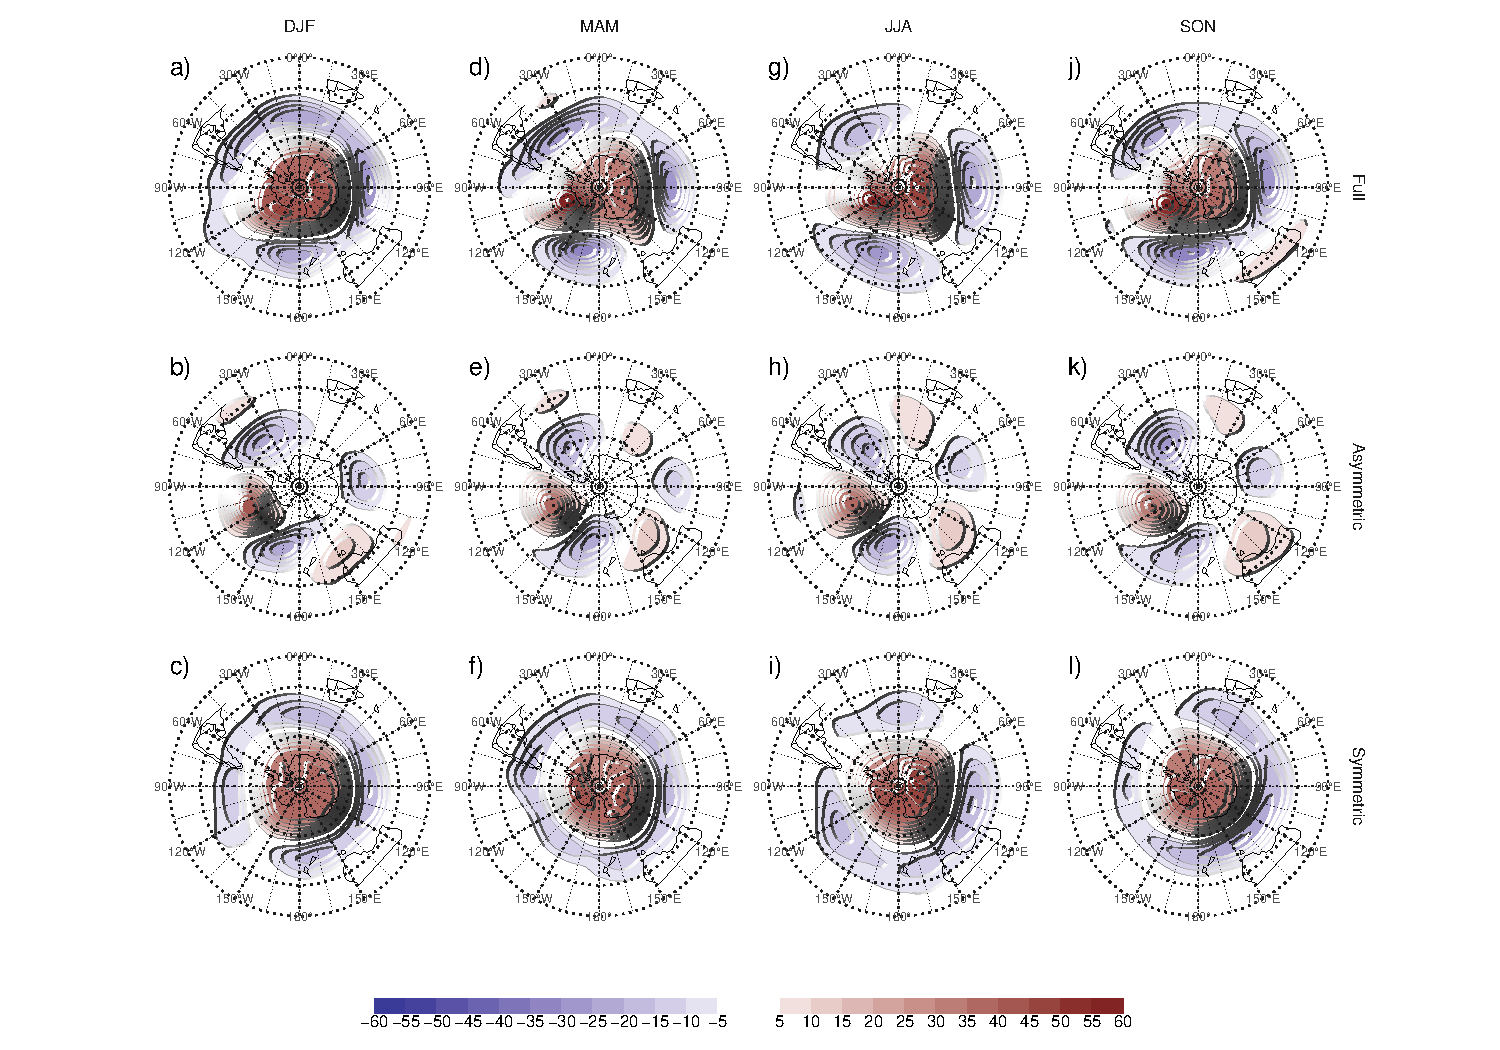
\includegraphics{2d-regr-700-1} \caption[Seasonal regression patterns of geopotential height at 700 hPa with the Full, Asymmetric and Symmetric SAM]{Seasonal regression patterns of geopotential height at 700 hPa with the Full, Asymmetric and Symmetric SAM. The regression patterns for Asymmetric and Symmetric SAM are the result of one multiple regression using both indices, not of two simple regressions involving each index by itsef.}\label{fig:2d-regr-700}
\end{sidewaysfigure}

\begin{figure}
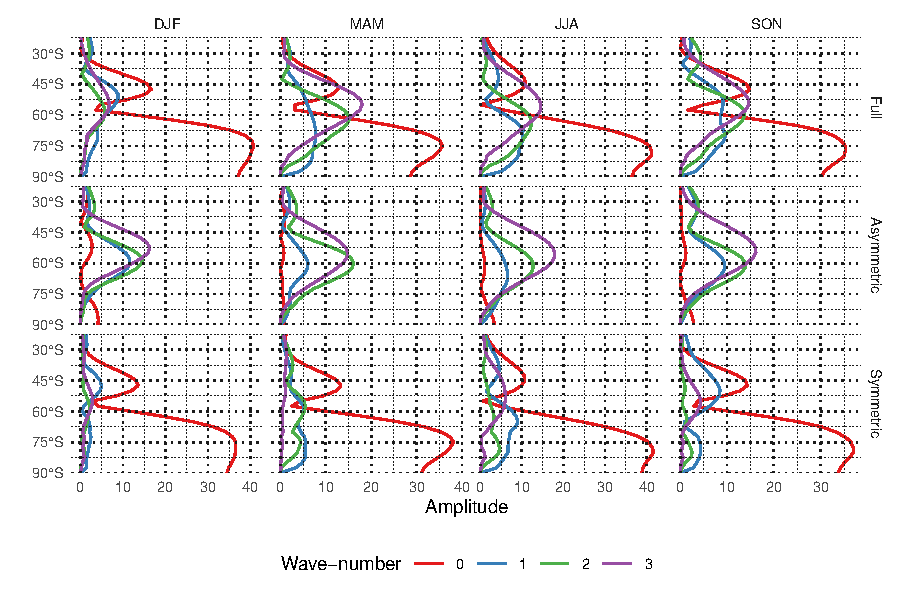
\includegraphics{wave-amplitude-700-1} \caption[Planteray wave amplitude for the regression patterns at 700 hPa]{Planteray wave amplitude for the regression patterns at 700 hPa.}\label{fig:wave-amplitude-700}
\end{figure}

\begin{sidewaysfigure}
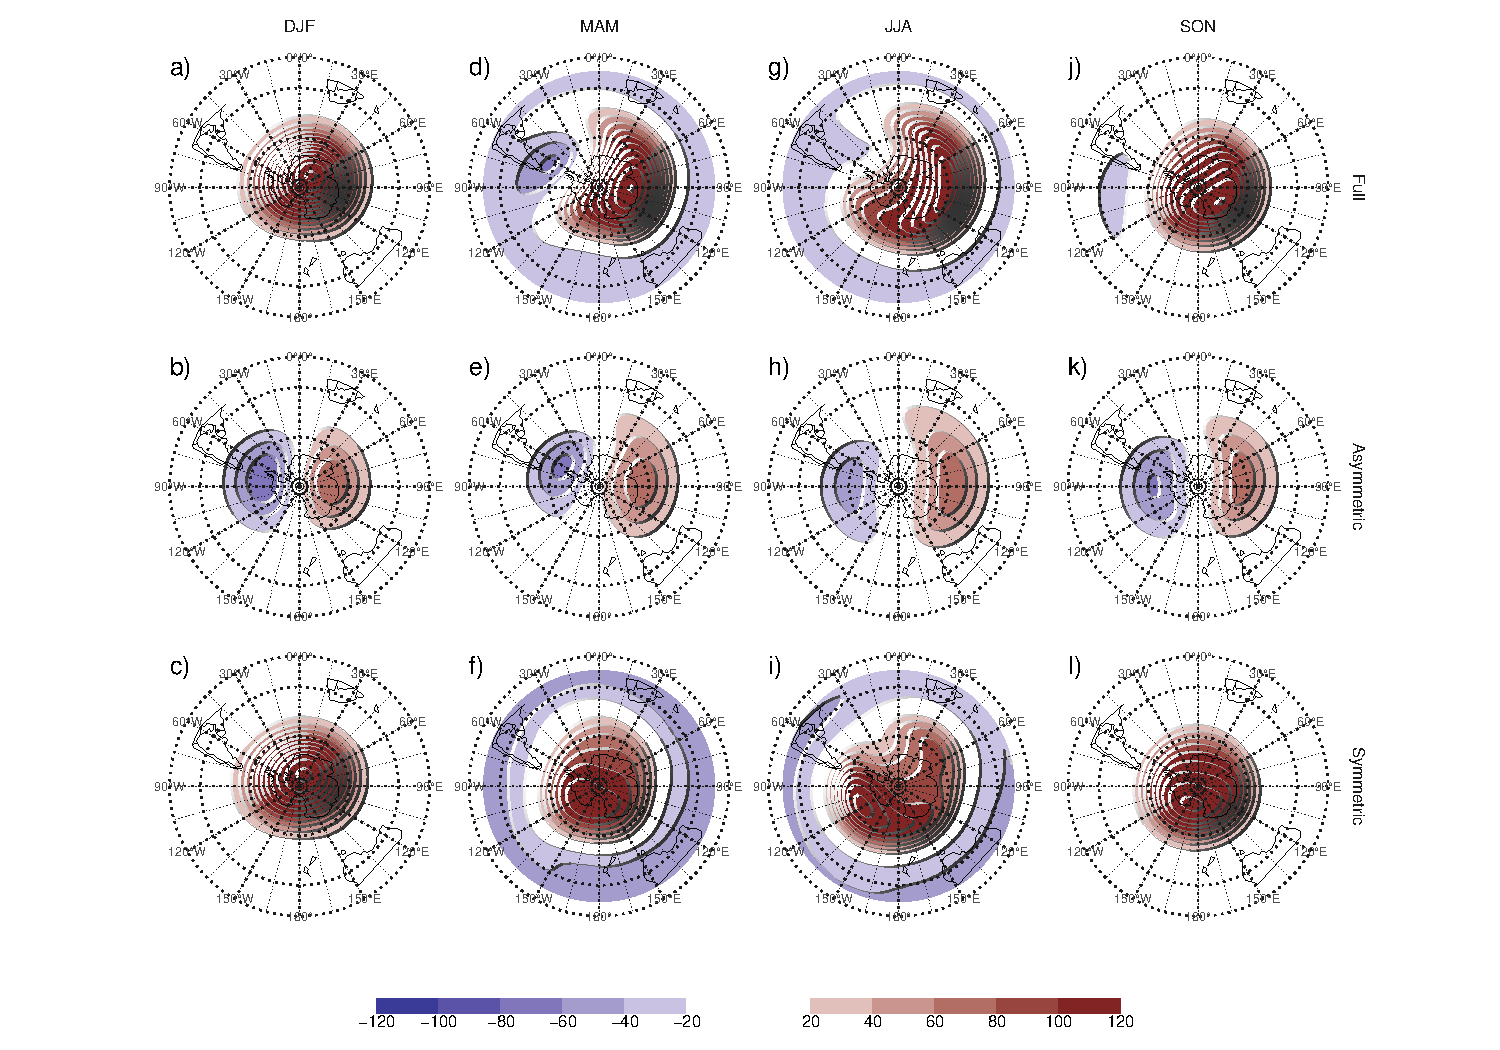
\includegraphics{2d-regr-30-1} \caption[Seasonal regression patterns of geopotential height at 30 hPa with the Full, Asymmetric and Symmetric SAM]{Seasonal regression patterns of geopotential height at 30 hPa with the Full, Asymmetric and Symmetric SAM. The regression patterns for Asymmetric and Symmetric SAM are the result of one multiple regression using both indices, not of two simple regressions involving each index by itsef.}\label{fig:2d-regr-30}
\end{sidewaysfigure}

\begin{figure}
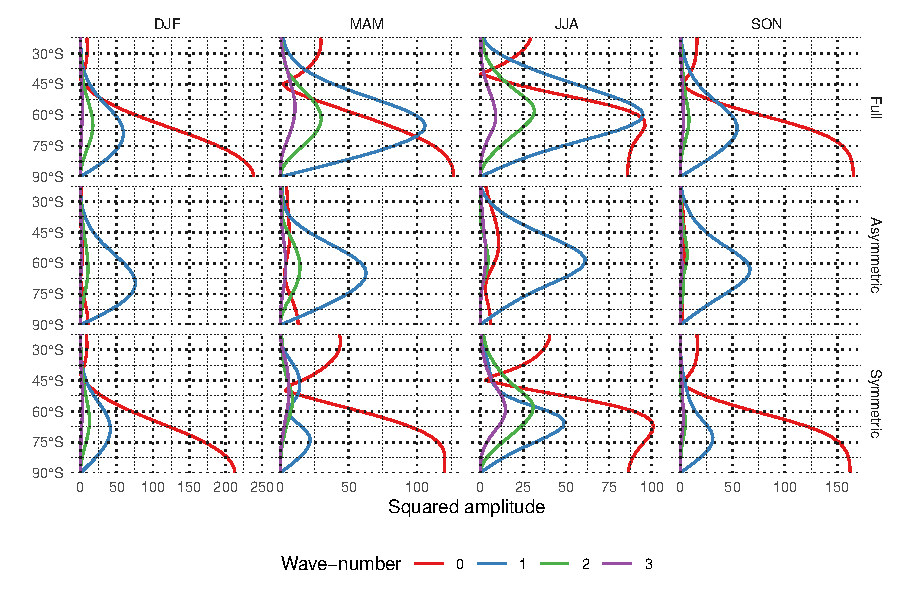
\includegraphics{wave-amplitude-30-1} \caption[Planteray wave amplitude for the regression patterns at 30 hPa]{Planteray wave amplitude for the regression patterns at 30 hPa.}\label{fig:wave-amplitude-30}
\end{figure}

\begin{sidewaysfigure}
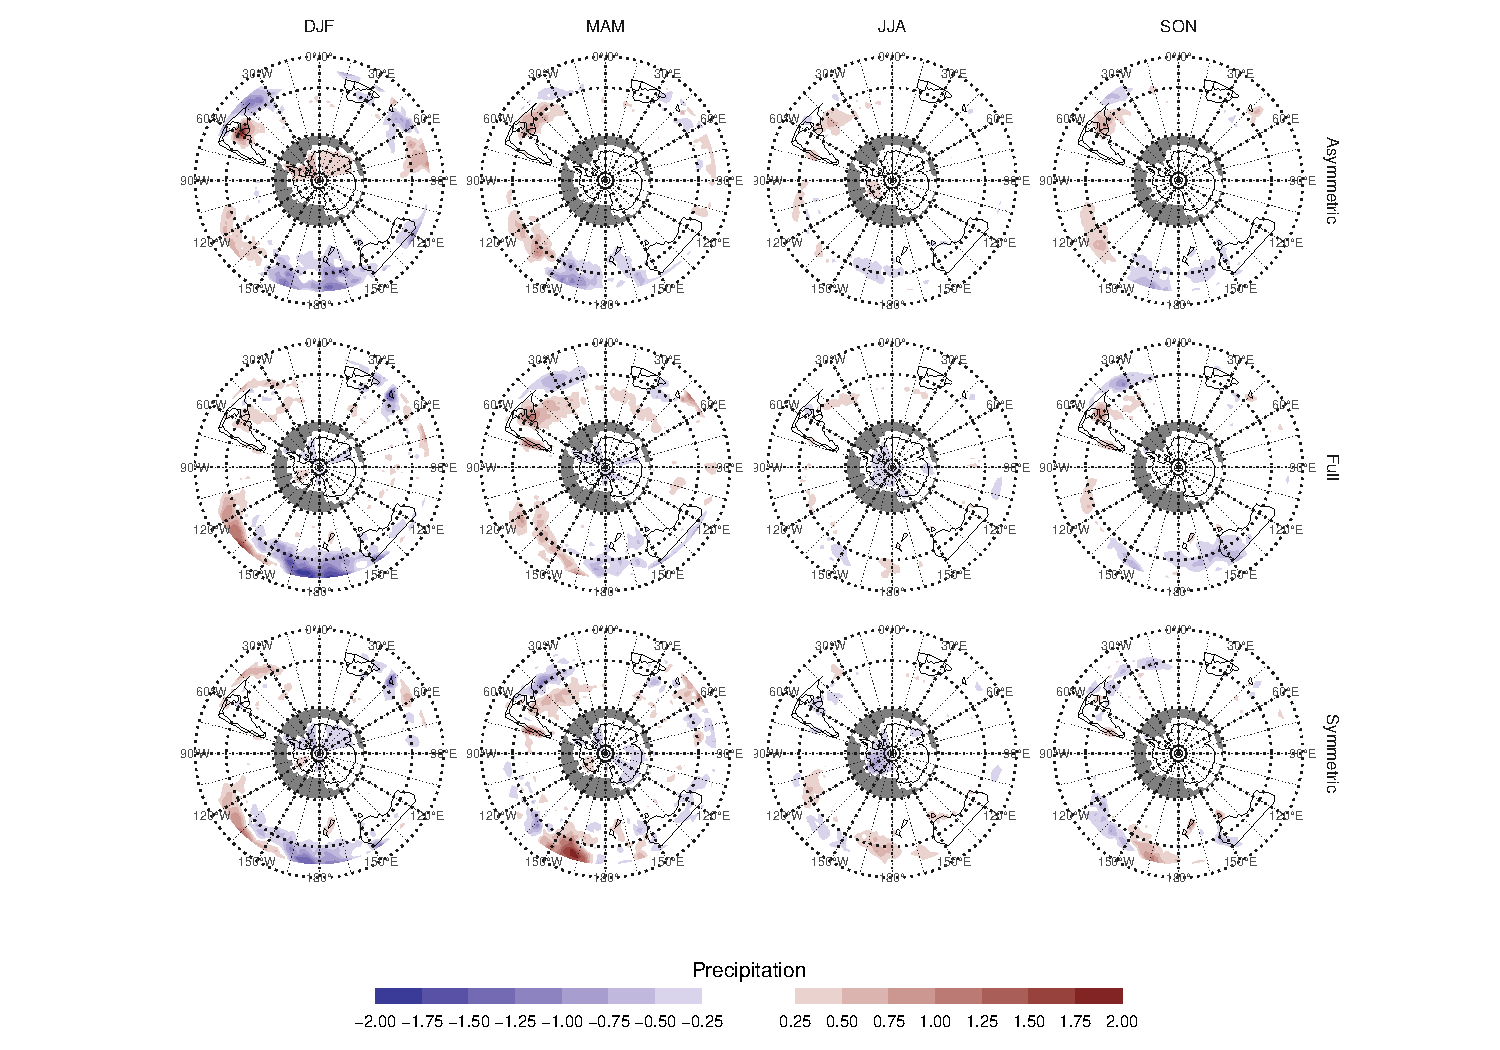
\includegraphics{pp-regr-global-1} \caption[Regression pattern of precipiation with Asymmetric and Symmetric SAM]{Regression pattern of precipiation with Asymmetric and Symmetric SAM. P-values smaller than 0.05 (controlling for Flase Detection Rate) as hatched areas.}\label{fig:pp-regr-global}
\end{sidewaysfigure}

\begin{sidewaysfigure}
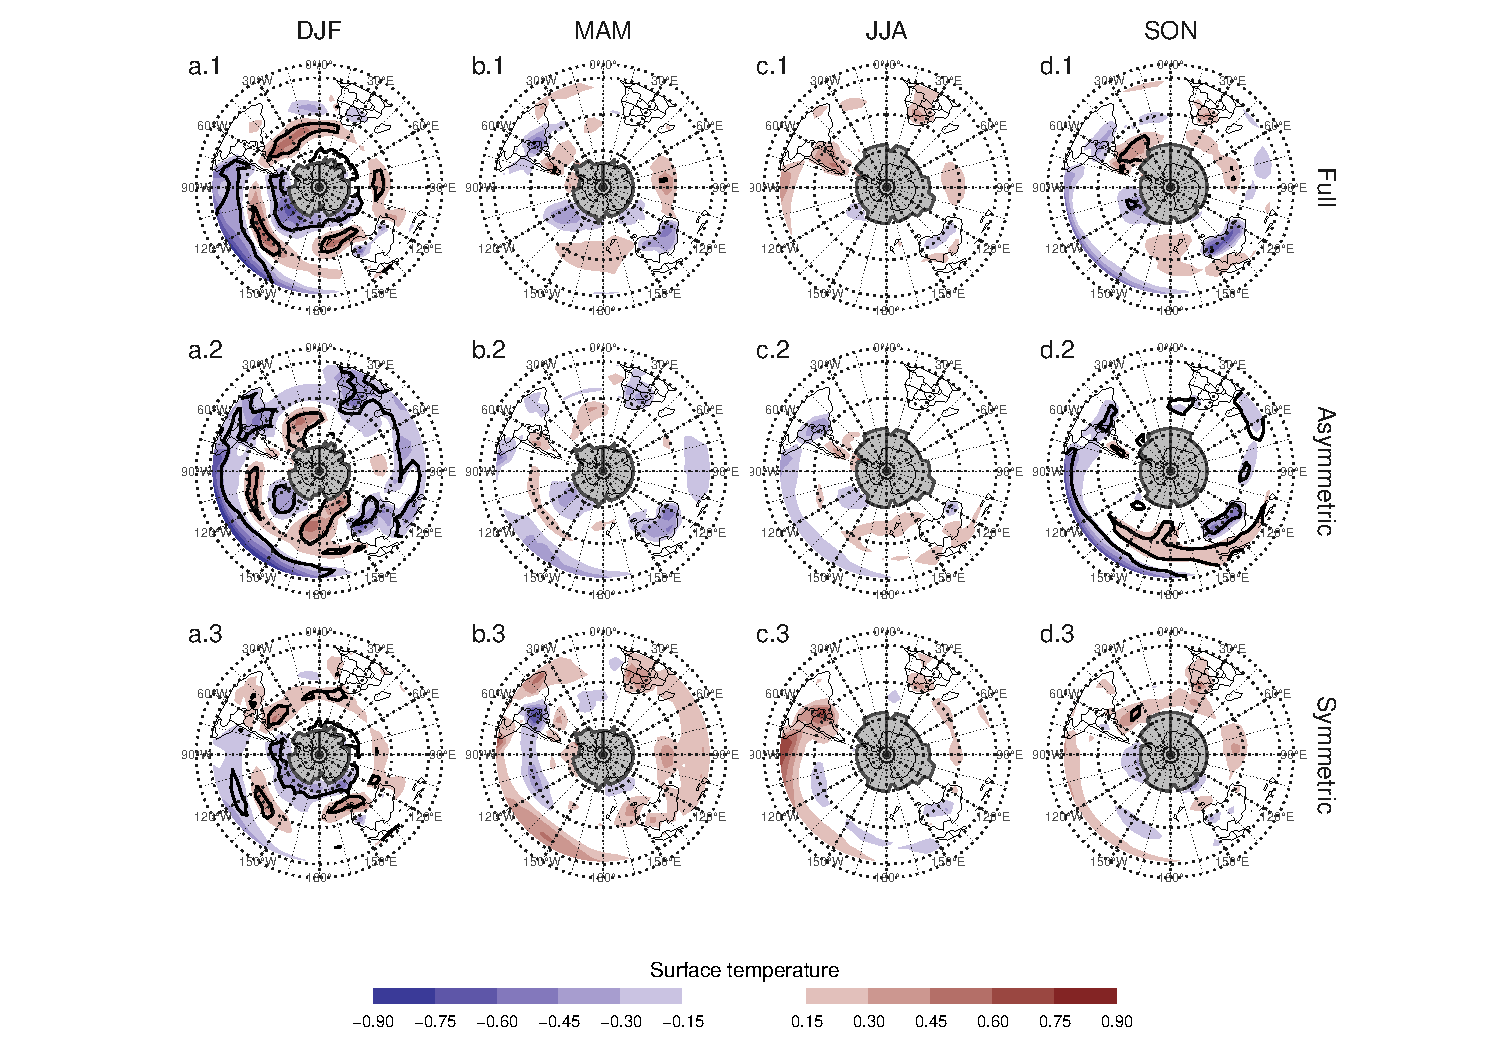
\includegraphics{regr-air-season-1} \caption[Regression pattern of surface temperature with Asymmetric and Symmetric SAM]{Regression pattern of surface temperature with Asymmetric and Symmetric SAM. P-values smaller than 0.05 (controlling for Flase Detection Rate) as hatched areas.}\label{fig:regr-air-season}
\end{sidewaysfigure}

\acknowledgments

CMAP Precipitation data provided by the NOAA/OAR/ESRL PSL, Boulder,
Colorado, USA, from their Web site at https://psl.noaa.gov/

NOAA Global Surface Temperature (NOAAGlobalTemp) data provided by the
NOAA/OAR/ESRL PSL, Boulder, Colorado, USA, from their Web site at
https://psl.noaa.gov/

\bibliography{AsymSAM}

\appendix

\appendixtitle{Extra figures}

\begin{figure}
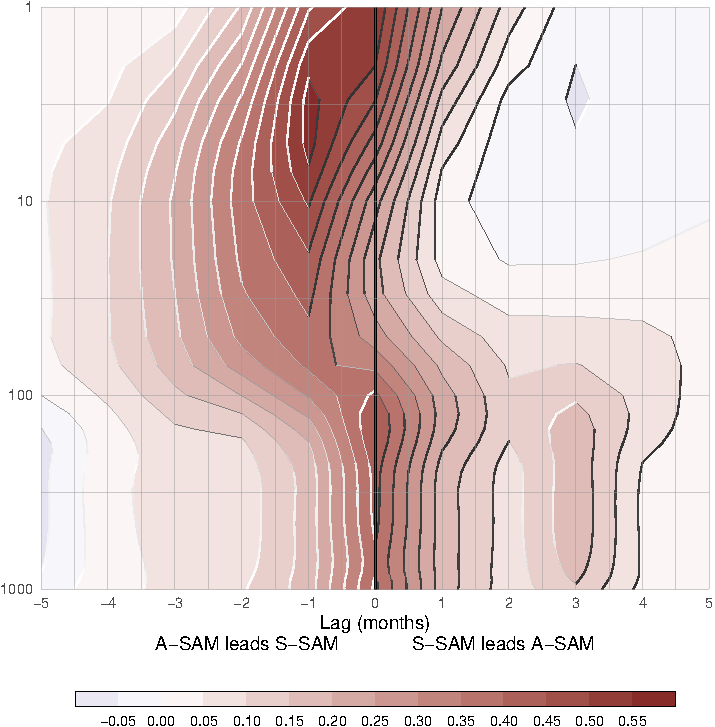
\includegraphics{A1-1} \appendcaption{A1}{Lag-correlation between Symmetric and Asymmetric SAM at each level.}\label{fig:A1}
\end{figure}

\begin{figure}
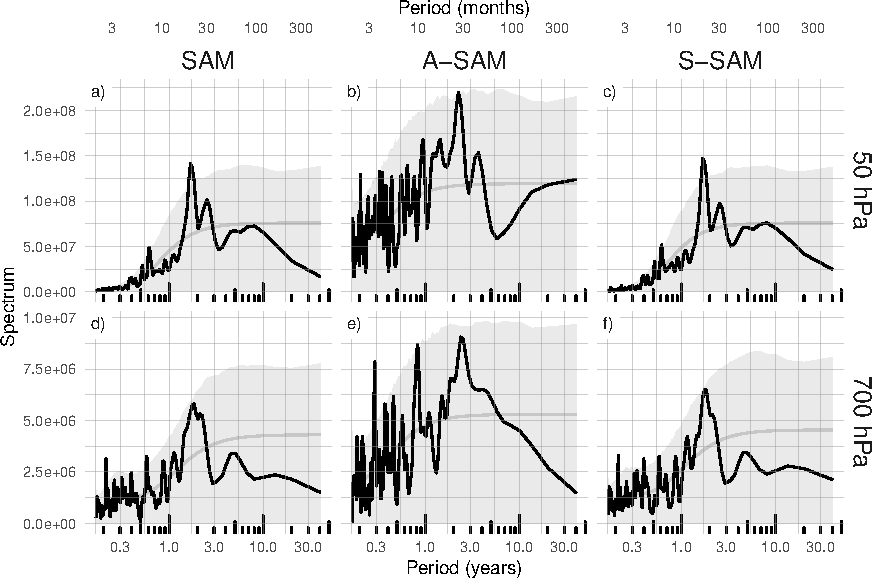
\includegraphics{A2-1} \appendcaption{A2}{Fourier spectrum of each timeseries. The shading indicates de 95\% qunatile derived fitting an AR process and bootstrapping 5000 simulated samples.}\label{fig:A2}
\end{figure}

\begin{figure}
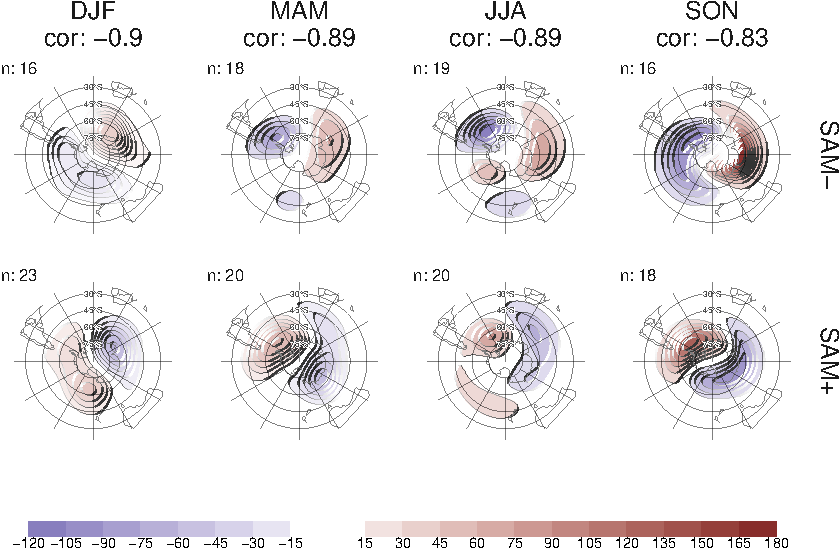
\includegraphics{A3-1} \appendcaption{A3}{Autocorrelation functions of each timeseries}\label{fig:A3}
\end{figure}

\begin{figure}
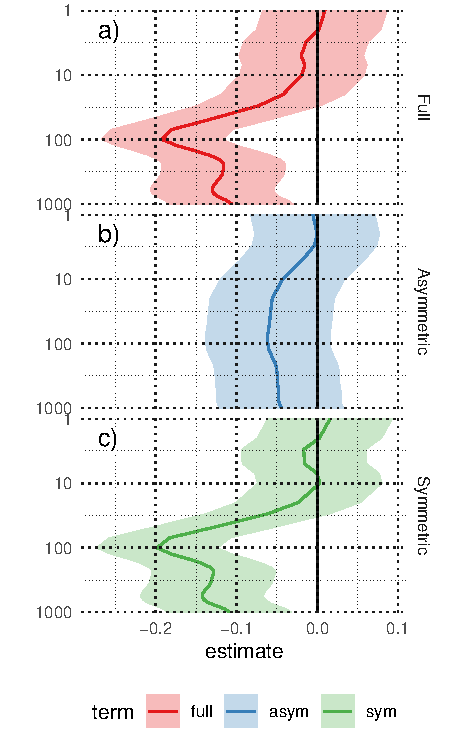
\includegraphics{A4-1} \appendcaption{A4}{Trends for each index at each level. Shading indicates the 95\% confidence interval.}\label{fig:A4}
\end{figure}


\end{document}
